\section{Empirical Results}
\label{sec:results}

This chapter reports the completed empirical evidence introduced in
Section~\ref{sec:research-design}. H2 is estimated using past-only P99
classifications and strictly ordered pre-trade and post-trade prices. The
expanding-history definition is primary and rolling-seven-day classification is
the principal definition robustness. All coefficients are conditional
associations; none identifies trader intent, private information, or a causal
effect.

\subsection{Descriptive statistics}

Table~\ref{tab:summary-statistics} reports summary statistics for the
dependent variable and the seven regressors used in the primary H1/H2
match-market models, computed on the 748,481-observation pre-kickoff sample.
The five-minute price change is highly concentrated at zero, consistent with
the 96.31\% zero-outcome share discussed below. Both flow variables are
signed-log transformed and are therefore approximately symmetric around a
small positive mean, reflecting a modest excess of buy-side over sell-side
pressure over the sample period.

Table~\ref{tab:correlation-matrix} reports pairwise Pearson correlations for
the same variables. These are descriptive associations only and are not
given a causal interpretation. Total net flow is mechanically related to its
large- and ordinary-trade components (correlations of 0.404 and 0.920
respectively) because total flow is the sum of the two; the three flow
measures are never included together in the same regression. Log lagged
30-minute volume and log minutes to kickoff are correlated at $-0.727$,
consistent with higher trading volume as kickoff approaches. All other
pairwise correlations among the model variables are below 0.21 in absolute
value. Notably, the five-minute price change itself is only weakly correlated
with the flow variables (0.135 for total flow, 0.139 for large flow, 0.094 for
ordinary flow) and is essentially uncorrelated with the baseline price, the
lagged price change, and the timing controls (all below 0.07 in absolute
value). This is consistent with a regression setting in which market and
calendar-hour fixed effects, rather than the raw pairwise correlations, do
most of the work of isolating the flow--price association reported below, and
it cautions against reading the simple correlations in Table~\ref{tab:correlation-matrix}
as a preview of the regression coefficients.

The P25, median, and P75 values for the large-flow variable in Table~\ref{tab:summary-statistics} are all zero, whereas the corresponding ordinary-flow values are strictly positive (0.693, 2.026, and 3.811 respectively). This asymmetry follows mechanically from the P99 classification rule: because a large trade occurs in at most about one per cent of trades within a market, most market-minutes record no large-trade activity at all, while ordinary trades are common enough that most market-minutes record some ordinary-trade flow. The non-zero minority of large-flow market-minutes is therefore what identifies the H2 large-flow coefficient, and the signed-log transformation compresses the tail of both variables without discarding it.

\begin{table}[htbp]
\centering
\caption{Summary statistics: primary pre-kickoff match-market sample}
\label{tab:summary-statistics}
\resizebox{\textwidth}{!}{%
\scriptsize
\begin{tabular}{lrrrrrrrr}
\hline
Variable & N & Mean & SD & Min & P25 & Median & P75 & Max \\
\hline
5-minute $\Delta$ YES-equivalent price & 748,481 & -0.000001 & 0.001460 & -0.090000 & 0.000000 & 0.000000 & 0.000000 & 0.060000 \\
Signed-log total net flow & 748,481 & 1.885274 & 3.174991 & -14.327927 & 0.693147 & 2.001480 & 3.813086 & 14.436413 \\
Signed-log P99 large-trade net flow & 748,481 & 0.026848 & 1.320026 & -14.335115 & 0.000000 & 0.000000 & 0.000000 & 14.423634 \\
Signed-log ordinary-trade net flow & 748,481 & 1.909488 & 2.995933 & -11.969488 & 0.693147 & 2.025513 & 3.810710 & 11.698710 \\
Baseline YES-equivalent price & 748,481 & 0.396755 & 0.238089 & 0.016500 & 0.205000 & 0.335000 & 0.595000 & 0.947000 \\
Lagged 30-minute price change & 748,481 & 0.000021 & 0.003011 & -0.090000 & 0.000000 & 0.000000 & 0.000000 & 0.100000 \\
Log lagged 30-minute volume & 748,481 & 6.529865 & 3.025122 & 0.000000 & 4.636717 & 6.771383 & 8.693629 & 15.831398 \\
Log minutes to kickoff & 748,481 & 7.360063 & 1.415594 & 1.791759 & 6.510258 & 7.445418 & 8.344267 & 10.567669 \\
\hline
\end{tabular}%
}
\par\vspace{4pt}
\noindent\begin{minipage}{\textwidth}
\footnotesize Notes: Statistics are computed on the 748,481-observation primary pre-kickoff match-market sample (312 match markets nested in 104 events, five-minute horizon). Flow variables are signed-log transformed: $\mathrm{sign}(\mathrm{flow})\times\log(1+|\mathrm{flow}|)$. Large trades are individual trades at or above their market-specific P99 threshold; ordinary trades are all remaining trades. These are descriptive statistics only and involve no hypothesis test.
\end{minipage}
\end{table}


\begin{table}[htbp]
\centering
\caption{Pairwise Pearson correlations: primary pre-kickoff match-market sample}
\label{tab:correlation-matrix}
\resizebox{\textwidth}{!}{%
\scriptsize
\begin{tabular}{lrrrrrrrr}
\hline
 & $\Delta$ price & Total flow & Large flow & Ordinary flow & Baseline price & Lag 30m $\Delta$ & Log lag vol. & Log min. to kickoff \\
\hline
$\Delta$ price & 1.000 & 0.135 & 0.139 & 0.094 & 0.007 & 0.067 & -0.002 & 0.002 \\
Total flow & 0.135 & 1.000 & 0.404 & 0.920 & 0.206 & -0.003 & 0.233 & -0.185 \\
Large flow & 0.139 & 0.404 & 1.000 & 0.101 & 0.064 & 0.015 & 0.043 & -0.037 \\
Ordinary flow & 0.094 & 0.920 & 0.101 & 1.000 & 0.206 & -0.019 & 0.258 & -0.213 \\
Baseline price & 0.007 & 0.206 & 0.064 & 0.206 & 1.000 & 0.022 & 0.141 & 0.145 \\
Lag 30m $\Delta$ & 0.067 & -0.003 & 0.015 & -0.019 & 0.022 & 1.000 & -0.009 & 0.013 \\
Log lag vol. & -0.002 & 0.233 & 0.043 & 0.258 & 0.141 & -0.009 & 1.000 & -0.727 \\
Log min. to kickoff & 0.002 & -0.185 & -0.037 & -0.213 & 0.145 & 0.013 & -0.727 & 1.000 \\
\hline
\end{tabular}%
}
\par\vspace{4pt}
\noindent\begin{minipage}{\textwidth}
\footnotesize Notes: Pairwise Pearson correlation coefficients computed on the 748,481-observation primary pre-kickoff match-market sample. Correlations are descriptive only and are not given a causal interpretation.
\end{minipage}
\end{table}


\subsection{Primary past-only P99 results}

Table~\ref{tab:v5-primary} reports the strictly aligned five-minute estimates.
The expanding-history sample contains 422,314 eligible market-minutes. The
large-flow coefficient is 0.000101 and the ordinary-flow coefficient is
0.000019; their difference is 0.000082 ($p<0.001$). The rolling-seven-day
sample contains 370,079 observations and produces the same large coefficient
(0.000101), a 0.000020 ordinary coefficient, and a 0.000081 difference
($p<0.001$). H2 is therefore supported under both past-only classifications.

Under the primary expanding-P99 signed-log specification, a
one-standard-deviation increase in the large-flow regressor corresponds to
approximately 0.0224 percentage points of five-minute probability movement,
compared with 0.0059 percentage points for ordinary flow. The
interquartile range of large flow is zero because most market-minutes contain no
P99 trade, so an interquartile-range effect is not informative for this sparse
regressor. These magnitudes are small: statistical precision should not be
confused with a large economic effect.

\begin{table}[htbp]
\centering
\caption{Past-only P99 five-minute directional-price results}
\label{tab:v5-primary}
\small
\begin{tabular}{lcc}
\toprule
 & Expanding history & Rolling seven day \\
\midrule
Large signed-log flow & 0.000101*** & 0.000101*** \\
 & (0.000008) & (0.000009) \\
Ordinary signed-log flow & 0.000019*** & 0.000020*** \\
 & (0.000003) & (0.000003) \\
Large minus ordinary & 0.000082*** & 0.000081*** \\
 & (0.000007) & (0.000007) \\
Observations & 422,314 & 370,079 \\
Markets & 252 & 236 \\
Match-event clusters & 104 & 103 \\
\bottomrule
\multicolumn{3}{p{0.92\textwidth}}{\footnotesize Notes: The outcome is the strictly aligned five-minute change in YES-equivalent probability. Both P99 definitions use only complete prior UTC days and require at least 1,000 prior within-market trades. Models include the stated controls, market and UTC calendar-hour fixed effects. CRV1 standard errors are clustered by match event. *** $p<0.01$.}
\end{tabular}
\end{table}


\subsection{Strict timing, lead--lag, and shared-event information}

Strict-0 alignment retains 748,372 of the 748,481 available five-minute rows;
strict-1 retains 748,420. The zero-change rate is 96.24\% under both rules.
Correcting the timing convention changes the five-minute outcome in 11,917
rows, but the H2 coefficient ordering is unchanged in strict-0, strict-1, and
above-median-volume market samples.

Within the eligible strict-0 samples, the recorded baseline precedes the focal
minute by a median of 56 seconds (maximum 58), while the five-minute outcome is
recorded a median of four seconds after its target (maximum 56); every retained
baseline and five-minute outcome is within 60 seconds of its target. As an
alternative to the CLOB history record, prices were reconstructed from executed
YES-equivalent trade prices, excluding the focal minute from the baseline. The
large-minus-ordinary contrast remains positive at 60-, 300-, and 900-second
matching tolerances: 0.000092--0.000091 under expanding history and
0.000087--0.000087 under rolling history (all $p<0.001$). Thus the main ordering
does not depend only on the price-history endpoint's recording mechanism,
although the primary outcome remains a recorded-price adjustment rather than a
quote-midpoint response.

The pre-specified lead--lag path in Table~\ref{tab:v5-leadlag} provides a more
direct timing diagnostic. Large-minus-ordinary contrasts at $-15$, $-5$, and
$-1$ minutes are close to zero and insignificant under both P99 definitions.
The contrast becomes positive at $+1$ minute and remains significant through
$+15$ minutes after Holm adjustment. At $+30$ minutes, expanding history passes
the five-per-cent threshold but rolling-seven-day does not, so continuation of
the post-trade association through 30 minutes is not definition-robust.

\begin{table}[htbp]
\centering
\caption{Pre-trade placebo and post-trade lead--lag contrasts}
\label{tab:v5-leadlag}
\small
\begin{tabular}{rcc}
\toprule
Horizon (minutes) & Expanding history & Rolling seven day \\
\midrule
$-15$ & $-0.0000005$ & $-0.0000028$ \\
$-5$  & $ 0.0000009$ & $ 0.0000004$ \\
$-1$  & $ 0.0000001$ & $-0.0000007$ \\
$+1$  & $ 0.0000581$*** & $ 0.0000580$*** \\
$+5$  & $ 0.0000815$*** & $ 0.0000814$*** \\
$+15$ & $ 0.0001078$*** & $ 0.0001052$*** \\
$+30$ & $ 0.0001186$** & $ 0.0001210$* \\
\bottomrule
\multicolumn{3}{p{0.92\textwidth}}{\footnotesize Notes: Entries are large-minus-ordinary coefficient contrasts. Negative horizons are pre-trade placebo outcomes. Stars use Holm-adjusted $p$-values across the seven horizons within each P99 definition: *** $p<0.01$, ** $p<0.05$, * $p<0.10$. Fixed effects and clustering follow Table~\ref{tab:v5-primary}.}
\end{tabular}
\end{table}


Figure~\ref{fig:v5-leadlag} displays the same estimates and confidence intervals.
The separation between the near-zero pre-trade coefficients and the positive
post-trade path is visible under both past-only definitions. Filled markers
denote horizons that remain significant after Holm adjustment; the rolling
seven-day estimate at $+30$ minutes is therefore left unfilled.

\begin{figure}[htbp]
\centering
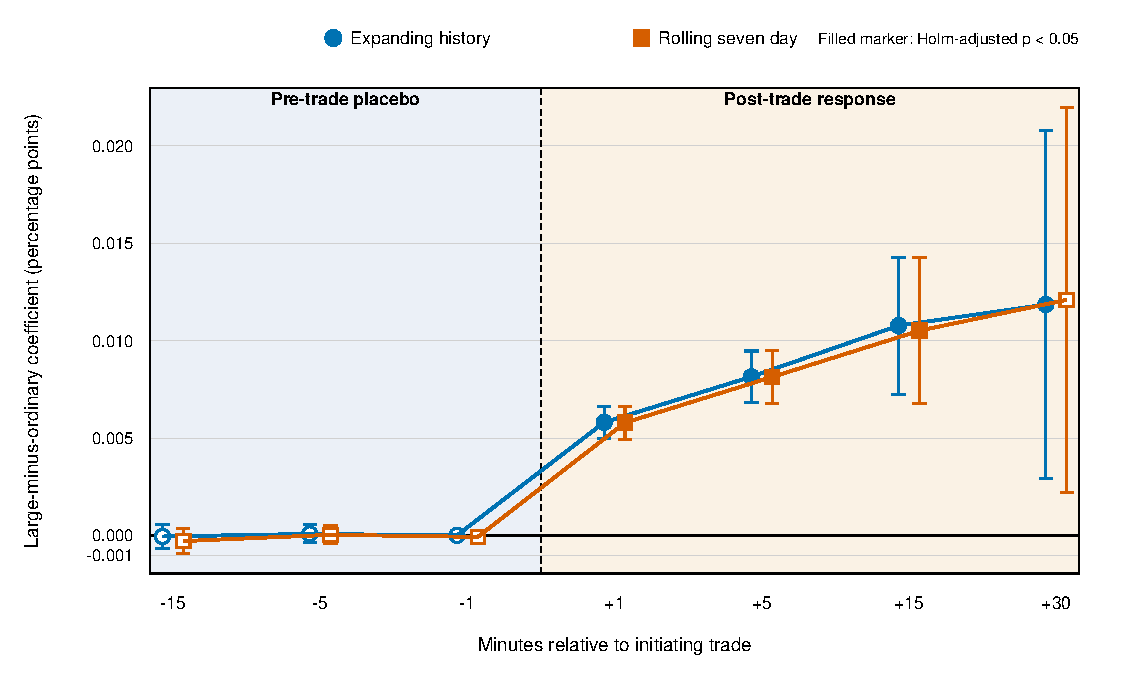
\includegraphics[width=0.90\textwidth]{figures/fig_v5_lead_lag.pdf}
\caption[Past-only lead--lag large-minus-ordinary coefficient path]{Past-only
large-minus-ordinary coefficient contrasts before and after the initiating
trade. Points show regression coefficients in percentage points and whiskers
show 95\% confidence intervals. Expanding-history and rolling-seven-day P99
thresholds use only complete prior UTC days. Filled markers indicate
Holm-adjusted $p<0.05$ within the seven-horizon family. Negative horizons are
pre-trade placebo outcomes; positive horizons are post-trade responses.}
\label{fig:v5-leadlag}
\end{figure}

Common match information does not eliminate the directional result. With
market and event-by-minute fixed effects, the contrast is 0.000102 under
expanding history and 0.000099 under rolling history; event-by-five-minute
estimates are 0.000074 and 0.000073. All four are significant at $p<0.001$.
These models compare related contracts within the same match-time cell and
therefore absorb match-level information shared at that resolution, but they do
not remove contract-specific responses to contemporaneous match news or
establish causality. The estimates therefore remain associational.

The extensive-margin evidence is less robust. Linear-probability models produce
positive large-minus-ordinary differences of 0.00641 (expanding) and 0.00605
(rolling), both significant. In converged market-fixed-effects logit models,
however, large and ordinary absolute flow are each positively associated with
update odds, while their difference is insignificant ($p=0.986$ and $p=0.511$).
Average marginal effects lead to the same conclusion. Under expanding history,
the large- and ordinary-flow marginal effects are 0.005615 and 0.005606, a
difference of 0.000008; under rolling history they are 0.005545 and 0.005894,
a difference of $-0.000349$. Thus, comparing effects on update probability does
not restore the linear-probability model's positive large-flow differential.
The claim that large flow is uniquely more likely to trigger an update is
therefore model-sensitive. Complementary log-log specifications did not produce
a stable finite solution and are not interpreted. Table~\ref{tab:v5-mechanism}
brings the extensive- and intensive-margin evidence together in the main
results. The conditional non-zero estimates are reported only descriptively
because the sample is selected on the realised outcome.

\begin{table}[htbp]
\centering
\caption{Update incidence and conditional non-zero price change}
\label{tab:v5-mechanism}
\small
\begin{tabular}{llcc}
\toprule
Outcome and model & Quantity reported & Expanding history & Rolling seven day \\
\midrule
Any update: LPM & Large-flow coefficient & 0.012176*** & 0.011847*** \\
 & Ordinary-flow coefficient & 0.005770*** & 0.005794*** \\
 & Large minus ordinary & 0.006406*** & 0.006052*** \\
\addlinespace
Any update: market-FE logit & Large-flow coefficient & 0.171711*** & 0.165123*** \\
 & Ordinary-flow coefficient & 0.171457*** & 0.175519*** \\
 & Large minus ordinary & 0.000254 & -0.010396 \\
 & Equality-test $p$-value & 0.986 & 0.511 \\
\addlinespace
Non-zero price change: OLS & Large minus ordinary & 0.000210*** & 0.000194*** \\
 & Selected observations & 17,994 & 17,270 \\
\bottomrule
\end{tabular}
\par\vspace{3pt}
\begin{minipage}{0.96\textwidth}
\footnotesize Notes: The first panel is a linear probability model for whether
any five-minute price update occurs. Logit coefficients in the second panel are
on the link scale and are not directly comparable in magnitude with LPM
coefficients; the focal test is equality of the large- and ordinary-flow
coefficients within each logit model. The final panel conditions on observing a
non-zero price change and is outcome-selected, so it is descriptive rather than
a primary mechanism test. All models use strict-0 timing, the stated controls,
market fixed effects, and event-clustered covariance. *** $p<0.01$.
\end{minipage}
\end{table}


\subsection{Subsequent continuation (H3a) and forecast improvement (H3b)}

Table~\ref{tab:h3} distinguishes subsequent movement from minute 5 to minute 15 (H3a) from ex-post forecast improvement (H3b). Both flow components predict continuation in the original direction. The large-minus-ordinary continuation difference is 0.000016 ($p=0.0065$), which is inconsistent with average reversal over the measured later interval, so H3a is supported. This is not strict persistence of an observed initial movement: when the initial five-minute price change is zero, the later movement may instead represent delayed adjustment. In the descriptive, outcome-selected sample restricted to a non-zero initial five-minute movement, the large-minus-ordinary differences are positive but insignificant under expanding history (0.000108, $p=0.161$) and rolling history (0.000085, $p=0.317$). The Brier-improvement coefficients are not statistically distinguishable from zero, and the corresponding large--ordinary equality tests are also insignificant, so H3b is not supported.

The large and ordinary signed-log coefficients are respectively 0.000033 and
0.000017 per one-unit change in their regressors; their difference is
0.0000161 ($p=0.0065$). This is a modest but statistically distinguishable
subsequent continuation association, not evidence of strict persistence. The
Brier-improvement equality tests are insignificant across the 0--5, 0--15 and
5--15 minute windows (minimum $p=0.138$), so H3b is not supported. Neither
result is evidence of informed trading, manipulation, or the absence of
manipulation; together they qualify the interpretation of the primary H2
directional association.

\begin{table}[htbp]
\centering
\caption{Persistence (H3a) and forecast-improvement (H3b) tests}
\label{tab:h3}
\scriptsize
\begin{tabular}{lccccc}
\hline
 & Subsequent total & Subsequent split & Brier 0--5 & Brier 0--15 & Brier 5--15 \\
\hline
Total signed flow & 0.000021*** &  &  &  &  \\
 & (0.000002) &  &  &  &  \\
P99 large flow &  & 0.000033*** &  &  &  \\
 &  & (0.000006) &  &  &  \\
Ordinary flow &  & 0.000017*** &  &  &  \\
 &  & (0.000002) &  &  &  \\
Absolute P99 large flow &  &  & 0.000000 & 0.000013 & 0.000012* \\
 &  &  & (0.000007) & (0.000012) & (0.000006) \\
Absolute ordinary flow &  &  & 0.000002 & 0.000005 & 0.000003 \\
 &  &  & (0.000003) & (0.000005) & (0.000003) \\
\hline
\multicolumn{6}{p{0.94\textwidth}}{\footnotesize Notes: Subsequent movement is $p_{t+15}-p_{t+5}$ conditional on the initial response. Positive Brier improvement denotes movement closer to the resolved outcome. All models use 744,470 observations and event-clustered CRV1 standard errors.}
\end{tabular}
\end{table}


\subsection{Timing and phase heterogeneity (RQ4)}

The joint tests in Table~\ref{tab:h4} reject equality of the pre-kickoff flow association across timing bands for both large and ordinary flow. The large-minus-ordinary difference is positive in every band, but the pattern is non-monotonic; it is smallest 6--12 hours before kickoff and largest during the final hour. Because RQ4 is exploratory rather than a directional hypothesis, this evidence answers the research question descriptively: the association varies significantly by time to kickoff, but not in a way that supports a claim that it continuously increases as kickoff approaches.

\begin{table}[htbp]
\centering
\caption{Time-to-kickoff heterogeneity (RQ4)}
\label{tab:h4}
\small
\begin{tabular}{lccc}
\hline
Time to kickoff & P99 large flow & Ordinary flow & Difference \\
\hline
$>24$ hours & 0.000190*** (0.000019) & 0.000081*** (0.000008) & 0.000108*** (0.000018) \\
12--24 hours & 0.000147*** (0.000017) & 0.000034*** (0.000005) & 0.000113*** (0.000015) \\
6--12 hours & 0.000091*** (0.000010) & 0.000024*** (0.000003) & 0.000067*** (0.000009) \\
1--6 hours & 0.000143*** (0.000018) & 0.000034*** (0.000005) & 0.000109*** (0.000015) \\
Final 60 minutes & 0.000163*** (0.000012) & 0.000022* (0.000012) & 0.000141*** (0.000016) \\
\hline
Joint interaction $F$ test & 11.019*** & 17.340*** &  \\
\hline
\multicolumn{4}{p{0.92\textwidth}}{\footnotesize Notes: Entries are pooled-model implied coefficients with clustered standard errors. Joint tests use $(4,103)$ degrees of freedom. The pattern is non-monotonic.}
\end{tabular}
\end{table}


Figure~\ref{fig:h4-timing} displays the same pattern graphically. The
large-flow coefficient exceeds the ordinary-flow coefficient in every band,
and the gap is not monotonic in time to kickoff: it narrows 6--12 hours
before kickoff before widening again in the final hour.

\begin{figure}[htbp]
\centering
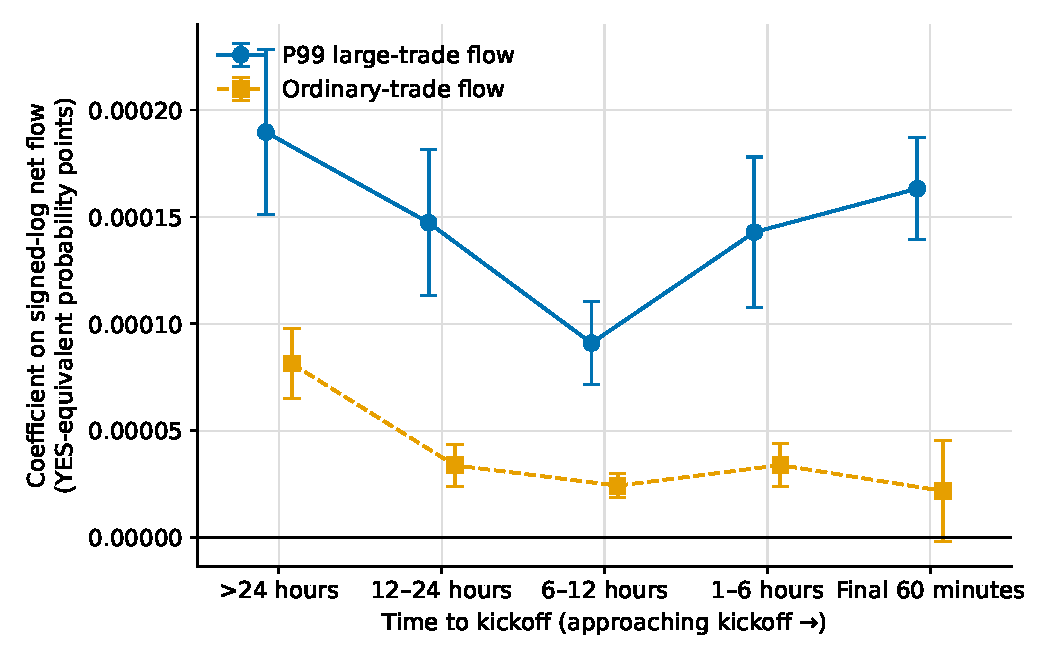
\includegraphics[width=0.85\textwidth]{figures/fig_2_h4_timing_large_vs_ordinary.pdf}
\caption[Large- versus ordinary-flow coefficients by time to kickoff]{Large- versus ordinary-flow coefficients across five pre-kickoff
time-to-kickoff bands, primary pre-kickoff match-market sample. Points are
implied marginal effects from the pooled interaction model with common
controls, market and calendar-hour fixed effects; error bars are 95\%
confidence intervals from CRV1 standard errors clustered by 104 match
events. The pattern is non-monotonic and is not interpreted as evidence of
informed trading or manipulation.}
\label{fig:h4-timing}
\end{figure}

RQ4's answer for pre-kickoff timing is that the signed-log flow--price association varies significantly across bands for both large and ordinary flow, with a large-minus-ordinary gap that is positive throughout but not monotonic in time to kickoff. The dip 6--12 hours before kickoff and the recovery in the final hour is an unexpected pattern relative to a simple story in which anticipation of the match builds steadily. One plausible explanation is the scheduled release of pre-match information, including team lineups, but because announcement timestamps are not observed in this dataset, this mechanism cannot be tested directly and no monotonic-approach-to-kickoff claim is supported.

Table~\ref{tab:phase} formally compares the pre-kickoff and post-kickoff/pre-resolution phases at the common five-minute horizon. Both the large- and ordinary-flow coefficients increase after kickoff, but the change in the large-minus-ordinary gap is not significant ($p=0.734$). RQ4's phase comparison therefore shows timing heterogeneity and a stronger overall post-kickoff flow--price association, but no phase-specific change in the relative large-trade premium. Post-kickoff estimates remain vulnerable to common shocks from goals, cards, substitutions, and VAR decisions.

\begin{table}[htbp]
\centering
\caption{Pre-/post-kickoff phase contrasts (RQ4)}
\label{tab:phase}
\small
\begin{tabular}{p{0.42\textwidth}rrrr}
\hline
Contrast & Estimate & SE & 95\% CI & $p$-value \\
\hline
Post-minus-prematch total-flow coefficient & 0.000546 & 0.000099 & [0.000351, 0.000742] & $<0.001$ \\
Prematch large-minus-ordinary & 0.000103 & 0.000012 & [0.000079, 0.000128] & $<0.001$ \\
Post-kickoff large-minus-ordinary & 0.000041 & 0.000187 & [-0.000329, 0.000411] & 0.826 \\
Post-minus-prematch large coefficient & 0.000416 & 0.000118 & [0.000182, 0.000649] & $<0.001$ \\
Post-minus-prematch ordinary coefficient & 0.000478 & 0.000131 & [0.000218, 0.000738] & $<0.001$ \\
Difference-in-differences: change in large-minus-ordinary gap & -0.000062 & 0.000183 & [-0.000424, 0.000300] & 0.734 \\
\hline
\multicolumn{5}{p{0.95\textwidth}}{\footnotesize Notes: The pooled five-minute sample contains 794,178 observations. Models use common controls, market and calendar-hour fixed effects, and CRV1 standard errors clustered by 104 events. Post-kickoff means before recorded resolution and is not necessarily purely in-play.}
\end{tabular}
\end{table}


\subsection{Country outright markets}

Table~\ref{tab:country} presents the separate secondary analysis of 48 country outright markets. At five minutes, the large-flow coefficient is 0.000091 and the ordinary-flow coefficient is 0.000017; their difference is significant ($p<0.001$). At thirty minutes, the respective coefficients are 0.000068 and 0.000016, with a difference-test $p$-value of 0.034. Excluding the four markets with fewer than five P99 trades changes the focal estimates by no more than about 0.06\%. Match and outright magnitudes are not directly comparable because their horizons, information environments, and clustering structures differ.

On this evidence, H2's large-versus-ordinary coefficient ordering is supported in the secondary country panel at both horizons, reinforcing the match-market conclusion in a structurally different set of markets without pooling the two families or treating the country result as an independent replication sample. Because these signed-log regressors have different distributions across the two market families, the country coefficients are not translated into a common raw-flow multiplier effect.

Because all 48 outright markets share tournament-level news, inference was also
recomputed with calendar-date clustering and two-way market-and-date covariance.
The five-minute large-minus-ordinary contrast is 0.000074 under market,
calendar-date, and two-way clustering; the corresponding $p$-values are below
$0.001$ in all three cases. This addresses observable calendar-time dependence
without converting the country extension into an independent replication.

\begin{table}[htbp]
\centering
\caption{Country outright-market regressions}
\label{tab:country}
\small
\begin{tabular}{lcccc}
\hline
 & 5m total & 5m split & 30m total & 30m split \\
\hline
Total flow & 0.000022*** &  & 0.000022** &  \\
 & (0.000004) &  & (0.000008) &  \\
P99 large flow &  & 0.000091*** &  & 0.000068** \\
 &  & (0.000014) &  & (0.000030) \\
Ordinary flow &  & 0.000017*** &  & 0.000016** \\
 &  & (0.000003) &  & (0.000007) \\
\hline
Observations & 646,607 & 646,607 & 645,157 & 645,157 \\
Market fixed effects & Yes & Yes & Yes & Yes \\
Calendar-hour fixed effects & Yes & Yes & Yes & Yes \\
\hline
\multicolumn{5}{p{0.94\textwidth}}{\footnotesize Notes: Country markets are separate secondary models. CRV1 standard errors are clustered by 48 markets. The 30-minute models use the common 5/30-minute sample.}
\end{tabular}
\end{table}


\subsection{Robustness checks and interpretation boundaries}
\label{sec:robustness-checks}

The principal robustness evidence is integrated above rather than presented as a
separate search across specifications. Strict-1 alignment produces the same
coefficient ordering as strict-0. Restricting the sample to 156
above-median-volume markets yields large-minus-ordinary contrasts of 0.0000803 under
expanding history and 0.0000805 under rolling history (both $p<0.001$). The
lead--lag placebo tests and event-by-time fixed effects address temporal ordering
and shared match shocks, while the logit comparison exposes functional-form
sensitivity in the update-incidence result.

The H2 ordering is also not unique to P99 or the signed-log transformation.
Across past-only P95, P97.5, P99, and P99.5 definitions, the large-minus-ordinary
contrast is positive and significant under both expanding and rolling histories
for signed-log, \texttt{asinh}, and winsorised raw flow scaled in \$1,000 units
(all 24 tests $p<0.001$). Under primary expanding P99, a one-standard-deviation
change implies 0.0224 percentage points for large flow and 0.0059 percentage
points for ordinary flow. At a common positive \$1,000 value, signed-log effects
are 0.0696 and 0.0133 percentage points; the winsorised raw-flow specification
gives 0.0181 and 0.0045 percentage points. The equality conclusion therefore
survives common scaling, although these alternative functional forms estimate
different response shapes.

Further covariance and
non-overlapping-window checks are retained in the appendix as secondary evidence.
All statistical significance denotes conditional association rather than a
causal effect, private information, institutional trading, manipulation, or a
market-integrity violation.

\subsection{Hypothesis decisions and unexpected findings}
\label{sec:hypothesis-decisions}

Table~\ref{tab:hypothesis-decisions} summarises the decision on each hypothesis alongside its key supporting evidence. H1 and H2 are supported as conditional associations, and the H2 contrast remains positive under both past-only classifications, strict timing, lead--lag diagnostics, and event-by-time fixed-effect specifications. The extensive-margin result is significant in linear probability models but not reproduced as a large-versus-ordinary difference in market-fixed-effects logit models. H3a and H3b are respectively supported and not supported. RQ4's descriptive answer is that timing and country-level heterogeneity are present but non-monotonic, while the post-/pre-kickoff phase-specific premium change is not significant.

\begin{table}[htbp]
\centering
\caption{Hypothesis decisions summary}
\label{tab:hypothesis-decisions}
\small
\begin{tabular}{p{0.24\textwidth}p{0.40\textwidth}p{0.28\textwidth}}
\hline
Hypothesis & Decision & Key evidence \\
\hline
H1 (baseline): total flow and short-horizon price & Supported (conditional association); validates the signed-flow construction & $\beta=0.000071$, $p<0.001$ \\ \hline
H2 (primary contribution): large- vs ordinary-flow association & Supported under both past-only definitions; extensive-margin interpretation is model-sensitive & Diff $=0.000082$ expanding and $0.000081$ rolling, both $p<0.001$; logit equality $p=0.986/0.511$ \\ \hline
H3a: persistence to minute 15 & Supported: no evidence of average reversal & Diff $=0.000016$, $p=0.007$ \\ \hline
H3b: forecast improvement (Brier) & Not supported & Brier tests n.s.\ (min $p=0.138$) \\ \hline
RQ4: timing and phase heterogeneity & Descriptive answer: timing association is significant but non-monotonic; phase-specific premium change not supported & Joint $F=11.019$/$17.340$, $p<0.001$; phase DiD $p=0.734$ \\ \hline
\multicolumn{3}{p{0.94\textwidth}}{\footnotesize Notes: All decisions describe conditional associations only. No decision implies a causal effect, informed trading, institutional trading, or a market-integrity violation. n.s.\ denotes not significant at the 5\% level.}
\end{tabular}
\end{table}


Three findings qualify a simple reading of the hypotheses. First, the
update-incidence interpretation is not reproduced by logit. Second, RQ4's timing
gap is non-monotonic. Third, both flow coefficients strengthen after kickoff,
but the large-minus-ordinary change is insignificant ($p=0.734$). Detailed MI,
HA, WH, machine-learning, and anomaly-screening results appear in
Appendix~\ref{sec:supplementary-integrity-results}. In brief, behavioural
features improve out-of-sample reversal prediction, while neither the
fixed-effects reversal tests nor the contextual review establish manipulation.
